\chapter{Point de vue Utilisateur}
\chaptermark{Utilisateur}

\section{Plugins développés}
\sectionmark{Plugins}
Middleware, notre plugin principal, propose la vue Eclipse suivante : 
  \begin{figure}[h]
	  \centering
	  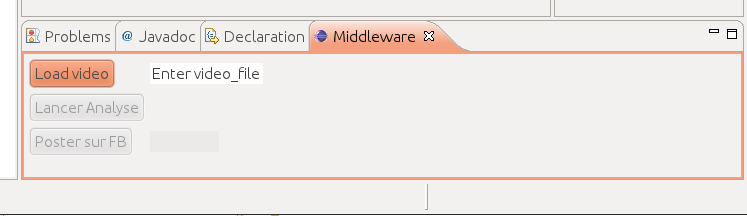
\includegraphics[scale=0.50]{img/Capture}
	  \caption{Vue du plugin}
	  \label{fig:vue}
\end{figure} 
\begin{description}
\item[Load Video]
L'utilisateur doit au préalable avoir renseigné le chemin de la vidéo à analyser. Le plugin Acquisition est sollicité au déclenchement de ce bouton. 
\item[Lancer Analyse]
Appel du plugin Reasoning qui effectue une analyse de la vidéo précedement acquise.
\item[Post]
L'utilisateur doit au préalable avoir renseigné l'acces token nécessaire pour poster sur une plateforme en ligne. 
Le plugin en charge de poster sur un blog ou un réseau social est appelé.
\end{description}
 
 \clearpage
 
\section{Lancement et manuel}
Pour lancer le plugin suivez les étape suivante:

\begin{enumerate}
 \item Dans le menu, cliquez sur \og Run \fg, puis sur \og Run configuration \fg, 
afin d'ouvrir une fenêtre de configuration (cf : \ref{fig:fenetreConfg} ).
  \item Une fois la fenêtre ouverte, cliquez sur l'onglet plugin et cochez les labels:
  \begin{enumerate}
      \item Acquisition
      \item Middleware
      \item NetP
      \item Reasoning
      \end{enumerate}
      \item Une fois les paramètres configurés cliquez sur \verb+Run+.
      \item Attendez que \emph{Eclipse} se lance. Lorsqu'\emph{Eclipse} sera lancé, allez dans \verb+Window+ $\rightarrow$ \verb+Show View+ $\rightarrow$ \verb+Other+\dots
      \item Choisissez \verb+middleware_view+ puis la vue \verb+Middleware+ (cf : \ref{fig:ShowView})
      \item Une fois que vous accès à la vue, entrez dans le premier champs de texte le chemin de la vidéo à analyser et cliquez sur\verb+LoadVideo+ afin de charger la vidéo
      \item Puis, pour lancer l'analyse, cliquez sur \verb+Lancer Analyse+
      \item Un fois l'analyse terminée, entrez le token associé à votre compte facebook pour cliquer sur \verb+ Poster sur FB+ une fois posté, le message sera envoyé sur facebook( cf \ref{fig:messageFB})
  \end{enumerate}
\begin{figure}[h]
	  \centering
	  
\includegraphics[scale=0.5]{img/cestlanuit}
	  \caption{Message sur Facebook}
	  \label{fig:messageFB}
\end{figure}
  \begin{figure}[h]
	  \centering
	  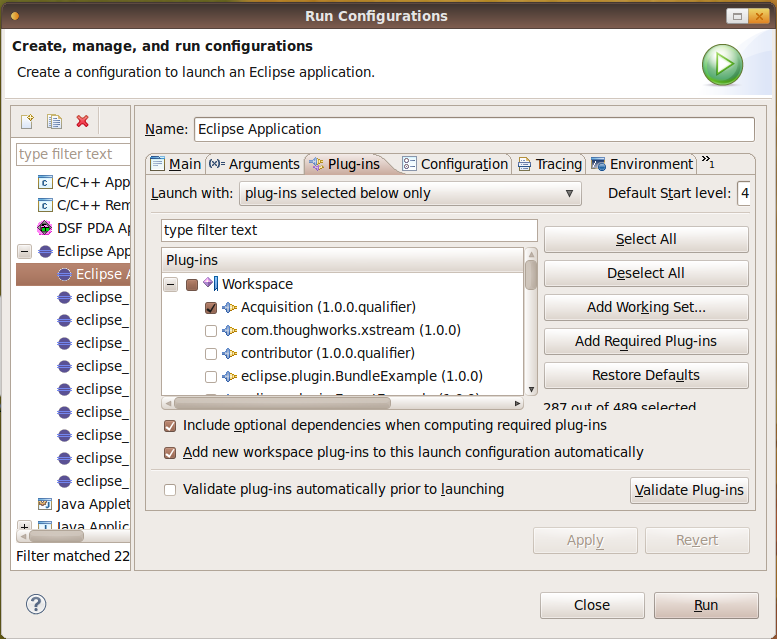
\includegraphics[scale=0.40]{img/tuto}
	  \caption{Fenêtre de configuration}
	  \label{fig:fenetreConfg}
\end{figure}
  \begin{figure}
	  \centering
	  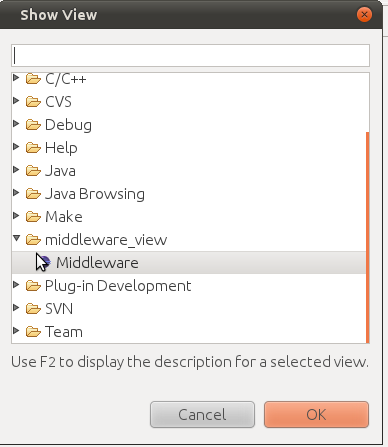
\includegraphics[scale=0.50]{img/ShowView}
	  \caption{Fenêtre Show View}
	  \label{fig:ShowView}
\end{figure}


